\documentclass[10pt]{beamer}

% ── Thème sobre ─────────────────────────────────────────────────────────
\usetheme{default}
\useinnertheme{rectangles}
\useoutertheme{infolines}

\definecolor{bleu}{RGB}{25,60,120}
\definecolor{bleulight}{RGB}{220,230,245}
\definecolor{gris}{RGB}{100,100,100}
\definecolor{bleudark}{RGB}{10,35,80}

\setbeamercolor{structure}{fg=bleu}
\setbeamercolor{frametitle}{fg=bleu, bg=bleulight}
\setbeamercolor{title}{fg=white, bg=bleu}
\setbeamercolor{subtitle}{fg=bleulight}
\setbeamercolor{author in head/foot}{bg=bleu, fg=white}
\setbeamercolor{title in head/foot}{bg=bleudark, fg=white}
\setbeamercolor{date in head/foot}{bg=bleu!70, fg=white}
\setbeamercolor{block title}{fg=white, bg=bleu}
\setbeamercolor{block body}{bg=bleulight!60}
\setbeamercolor{block title alerted}{fg=white, bg=bleu!70!black}
\setbeamercolor{block body alerted}{bg=bleulight!40}
\setbeamercolor{itemize item}{fg=bleu}
\setbeamercolor{itemize subitem}{fg=bleu!60}
\setbeamercolor{enumerate item}{fg=bleu}

\setbeamerfont{frametitle}{series=\bfseries, size=\large, family=\rmfamily}
\setbeamerfont{title}{series=\bfseries, size=\Large, family=\rmfamily}
\setbeamerfont{block title}{series=\bfseries, family=\rmfamily}
\setbeamerfont{normal text}{family=\rmfamily}

\setbeamertemplate{navigation symbols}{}
\setbeamertemplate{itemize item}{$\bullet$}
\setbeamertemplate{itemize subitem}{$\circ$}

% ── Packages ────────────────────────────────────────────────────────────
\usepackage[utf8]{inputenc}
\usepackage[T1]{fontenc}
\usepackage{lmodern}
\usepackage{amsmath, amssymb}
\usepackage{mathtools}
\usepackage{tikz}
\usetikzlibrary{arrows.meta, positioning, decorations.pathreplacing, calc}
\usepackage{booktabs}
\usepackage{listings}
\usepackage{xcolor}
\definecolor{bleu}{RGB}{0,114,189}
\definecolor{gris}{gray}{0.5}

\lstset{
	language=Python,
	basicstyle=\ttfamily\scriptsize,
	keywordstyle=\color{bleu}\bfseries,
	commentstyle=\color{gris}\itshape,
	stringstyle=\color{bleu!70!black},
	backgroundcolor=\color{bleulight!50},
	frame=single, framerule=0.4pt,
	rulecolor=\color{bleu!40},
	numbers=left, numberstyle=\tiny\color{gris},
	breaklines=true, showstringspaces=false
}

% ── Macros ──────────────────────────────────────────────────────────────
\newcommand{\scalaire}[2]{\langle #1,\, #2 \rangle}
\newcommand{\norme}[1]{\left\| #1 \right\|}
\newcommand{\RR}{\mathbb{R}}
\newcommand{\ZZ}{\mathbb{Z}}
\renewcommand{\d}{\,\mathrm{d}}

% ── Titre ───────────────────────────────────────────────────────────────
\title{Compression d'image par ondelettes}
\subtitle{De l'analyse de Fourier à la transformée en ondelettes discrète}
\author{De~Haese~Tao \and Piémontèse~Enzo \and Thirion~Louis}
\institute{Cité scolaire Carnot}
\date{TIPE 2025}

% ════════════════════════════════════════════════════════════════════════
\begin{document}
	% ════════════════════════════════════════════════════════════════════════
	
	\begin{frame}
		\titlepage
	\end{frame}
	
	% ── Plan ─────────────────────────────────────────────────────────────────
	\begin{frame}{Plan}
		\tableofcontents
	\end{frame}
	
	% ════════════════════════════════════════════════════════════════════════
	\section{I. Au-delà de l'analyse de Fourier}
	% ════════════════════════════════════════════════════════════════════════
	
	\begin{frame}{I — Le problème de Fourier}
		
		La transformée de Fourier d'une fonction $f \in L^1(\RR)$ est :
		\[
		\hat{f}(\nu) = \int_{-\infty}^{+\infty} f(x)\, e^{-2i\pi\nu x} \d x
		\]
		
		\medskip
		\textbf{Puissance} : décomposition fréquentielle complète et inversible.
		
		\medskip
		\textbf{Limite fondamentale} : les fonctions analysantes $x \mapsto e^{2i\pi\nu x}$
		sont \emph{de support infini} — elles ne sont pas localisées.
		
		\medskip
		\begin{block}{Conséquence}
			Un événement ponctuel (discontinuité, transitoire) à la position $x_0$
			affecte $\hat{f}(\nu)$ \emph{pour toutes} les fréquences $\nu$.
			On ne peut pas savoir \emph{où} dans le signal un phénomène se produit.
		\end{block}
		
	\end{frame}
	
	% ─────────────────────────────────────────────────────────────────────────
	\begin{frame}{I — Illustration : localisation et Fourier}
		
		\begin{columns}[T]
			\column{0.50\textwidth}
			\textbf{Signal composé de deux sinusoïdes successives}
			
			\begin{center}
				\begin{tikzpicture}[scale=0.75]
					% Signal : sin basse fréq sur [0, 0.5], sin haute fréq sur [0.5, 1]
					\draw[->] (0,0) -- (5.2,0) node[right] {\small $x$};
					\draw[->] (0,-1.3) -- (0,1.5) node[above] {\small $f(x)$};
					% basse freq : 2 oscillations sur [0,2.5]
					\foreach \i in {0,...,3} {
						\draw[bleu, thick, domain=0:1.25, samples=30]
						plot ({0.625*\i+\x*0.625}, {sin(360*2*\x/1 r)});
					}
					% haute freq : 8 oscillations sur [2.5,5]
					\foreach \i in {0,...,7} {
						\draw[bleu!50!black, thick, domain=0:0.625, samples=20]
						plot ({2.5+0.3125*\i+\x*0.3125}, {0.8*sin(360*\x r)});
					}
					\draw[dashed, gris] (2.5,-1.2) -- (2.5,1.2);
					\node[below, gris, font=\footnotesize] at (2.5,0) {$x_0$};
					\node[font=\tiny, bleu] at (1.25,1.3) {basse fréq.};
					\node[font=\tiny, bleu!50!black] at (3.75,1.0) {haute fréq.};
				\end{tikzpicture}
			\end{center}
			
			\column{0.46\textwidth}
			\textbf{Module de la TF}
			
			\begin{center}
				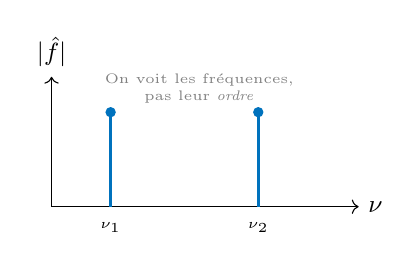
\begin{tikzpicture}[scale=0.75]
					\draw[->] (0,0) -- (5.2,0) node[right] {\small $\nu$};
					\draw[->] (0,0) -- (0,2.2) node[above] {\small $|\hat{f}|$};
					% Deux pics, mais impossible de savoir qu'ils sont successifs
					\draw[bleu, very thick] (1.0,0) -- (1.0,1.6);
					\fill[bleu] (1.0,1.6) circle (2.5pt);
					\draw[bleu, very thick] (3.5,0) -- (3.5,1.6);
					\fill[bleu] (3.5,1.6) circle (2.5pt);
					\node[font=\tiny, below] at (1.0,-0.1) {$\nu_1$};
					\node[font=\tiny, below] at (3.5,-0.1) {$\nu_2$};
					\node[font=\tiny, gris, align=center] at (2.5,2.0)
					{On voit les fréquences,\\pas leur \emph{ordre}};
				\end{tikzpicture}
			\end{center}
			
			\medskip
			La TF révèle que les fréquences $\nu_1$ et $\nu_2$ sont présentes,
			mais \emph{pas} qu'elles apparaissent l'une après l'autre.
		\end{columns}
		
	\end{frame}
	
	% ─────────────────────────────────────────────────────────────────────────
	\begin{frame}{I — La solution : une \og petite onde \fg}
		
		\textbf{Idée} : remplacer les sinusoïdes infinies par des fonctions
		\emph{oscillantes et localisées}.
		
		\medskip
		\begin{block}{Définition — Ondelette mère}
			Une fonction $\psi \in L^2(\RR)$ est une \emph{ondelette} si elle vérifie
			la condition d'admissibilité :
			\[
			C_\psi = \int_0^{+\infty} \frac{|\hat{\psi}(\nu)|^2}{\nu} \d\nu < +\infty,
			\]
			ce qui implique en particulier $\displaystyle\int_{\RR} \psi(x)\d x = 0$
			(moyenne nulle --- \emph{oscillation}).
		\end{block}
		
		\medskip
		À partir de $\psi$, on construit une famille par \textbf{dilatation} (échelle $a$)
		et \textbf{translation} (position $b$) :
		\[
		\psi_{a,b}(x) = \frac{1}{\sqrt{a}}\,\psi\!\left(\frac{x - b}{a}\right),
		\quad a > 0,\; b \in \RR.
		\]
		Le facteur $\tfrac{1}{\sqrt{a}}$ assure la conservation de l'énergie :
		$\norme{\psi_{a,b}} = \norme{\psi}$.
		
	\end{frame}
	
	% ════════════════════════════════════════════════════════════════════════
	\section{II. Cadre mathématique}
	% ════════════════════════════════════════════════════════════════════════
	
	\begin{frame}{II — L'espace $L^2(\RR)$ et le produit scalaire}
		
		\begin{block}{Espace de travail}
			\[
			L^2(\RR) = \left\{ f : \RR \to \RR \;\Big|\; \int_\RR |f(x)|^2 \d x < +\infty \right\}
			\]
			C'est un espace de Hilbert pour le produit scalaire
			$\scalaire{f}{g} = \displaystyle\int_\RR f(x)\, g(x) \d x$.
		\end{block}
		
		\medskip
		\textbf{Énergie d'un signal} : $E(f) = \norme{f}^2 = \scalaire{f}{f}$.
		
		\medskip
		\textbf{Identité de Parseval} : pour toute base orthonormée $(e_k)$ de $L^2(\RR)$,
		\[
		\norme{f}^2 = \sum_k |\scalaire{f}{e_k}|^2.
		\]
		
		\medskip
		\begin{alertblock}{Lien avec le programme de MP}
			$L^2(\RR)$ est le complété de l'espace préhilbertien des fonctions continues
			à support compact. Le théorème de représentation de Riesz garantit que toute
			forme linéaire continue s'écrit comme un produit scalaire.
		\end{alertblock}
		
	\end{frame}
	
	% ─────────────────────────────────────────────────────────────────────────
	\begin{frame}{II — L'ondelette mère et la fonction d'échelle}
		
		\begin{columns}[T]
			\column{0.50\textwidth}
			
			\begin{block}{Ondelette mère $\psi$}
				Capture les \textbf{détails}, les oscillations et les singularités.
				\[
				\int_\RR \psi(x)\d x = 0 \quad (\text{moyenne nulle})
				\]
				Coefficient d'ondelette :
				\[
				d_{j,k} = \scalaire{f}{\psi_{j,k}} = \int_\RR f(x)\,\psi_{j,k}(x)\d x
				\]
				\emph{Mesure le contenu de $f$ à l'échelle $2^{-j}$
					autour de la position $k \cdot 2^{-j}$.}
			\end{block}
			
			\column{0.46\textwidth}
			
			\begin{block}{Fonction d'échelle $\varphi$}
				Capture la \textbf{tendance globale}, la moyenne locale.
				\[
				\int_\RR \varphi(x)\d x = 1 \quad (\text{moyenne non nulle})
				\]
				Coefficient d'approximation :
				\[
				c_{j,k} = \scalaire{f}{\varphi_{j,k}} = \int_\RR f(x)\,\varphi_{j,k}(x)\d x
				\]
				\emph{Représente $f$ lissée à la résolution $2^{-j}$.}
			\end{block}
			
		\end{columns}
		
		\medskip
		\begin{center}
			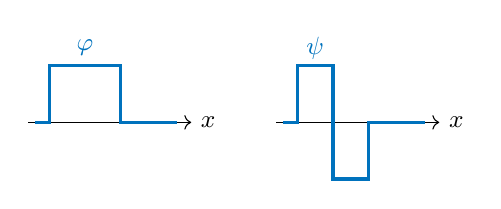
\begin{tikzpicture}[scale=0.9]
				% phi : créneau positif
				\draw[->] (-0.3,0) -- (2.0,0) node[right] {\small $x$};
				\draw[bleu, very thick] (-0.2,0)--(-0.0,0)--(0,0.8)--(1,0.8)--(1,0)--(1.8,0);
				\node[bleu, font=\small] at (0.5,1.05) {$\varphi$};
				% psi : créneau +/- à droite
				\begin{scope}[xshift=3.5cm]
					\draw[->] (-0.3,0) -- (2.0,0) node[right] {\small $x$};
					\draw[bleu, very thick]
					(-0.2,0)--(0,0)--(0,0.8)--(0.5,0.8)--(0.5,-0.8)--(1,-0.8)--(1,0)--(1.8,0);
					\node[bleu, font=\small] at (0.25,1.05) {$\psi$};
				\end{scope}
			\end{tikzpicture}
			\quad \small (exemple : Haar)
		\end{center}
		
	\end{frame}
	
	% ─────────────────────────────────────────────────────────────────────────
	\begin{frame}{II — Construction de la base : dilatations et translations}
		
		À partir de $\psi$, on définit pour $j \in \ZZ$, $k \in \ZZ$ :
		\[
		\boxed{\psi_{j,k}(x) = 2^{j/2}\,\psi(2^j x - k)}
		\]
		
		\begin{columns}[T]
			\column{0.48\textwidth}
			
			\medskip
			\textbf{Rôle des paramètres :}
			\begin{itemize}
				\item $j$ contrôle l'\textbf{échelle} : $j$ grand $\Rightarrow$ fenêtre fine,
				haute fréquence
				\item $k$ contrôle la \textbf{position} : décalage de $k \cdot 2^{-j}$
				\item Le facteur $2^{j/2}$ normalise : $\norme{\psi_{j,k}} = 1$
			\end{itemize}
			
			\medskip
			\begin{block}{Théorème (base de Haar)}
				$\{\varphi(\cdot - k),\; \psi_{j,k}\}_{j \geq 0,\, k \in \ZZ}$ est une
				base hilbertienne de $L^2(\RR)$ :
				\[
				f = \sum_k c_k\,\varphi(\cdot-k) + \sum_{j \geq 0}\sum_k d_{j,k}\,\psi_{j,k}
				\]
			\end{block}
			
			\column{0.48\textwidth}
			
			\begin{center}
				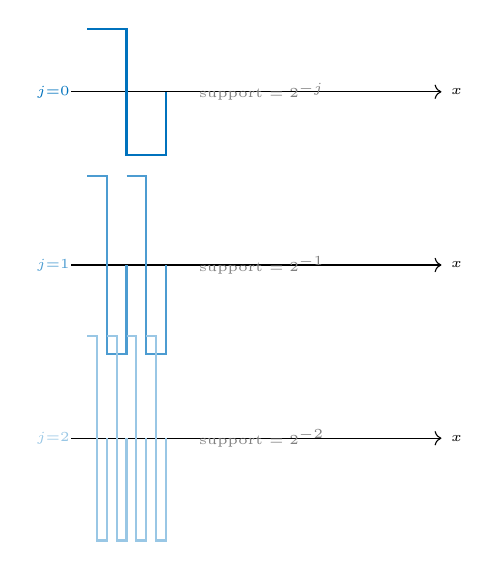
\begin{tikzpicture}[scale=1.0]
					% j=0 : psi_{0,0}, support [0,1]
					\draw[->] (-0.2,0) -- (4.5,0) node[right] {\tiny $x$};
					\draw[bleu, thick]
					(0,0.8)--(0.5,0.8)--(0.5,-0.8)--(1,-0.8)--(1,0);
					\node[bleu, left, font=\tiny] at (-0.1,0) {$j{=}0$};
					
					% j=1 : psi_{1,0} support [0,0.5], hauteur sqrt(2)
					\begin{scope}[yshift=-2.2cm]
						\draw[->] (-0.2,0) -- (4.5,0) node[right] {\tiny $x$};
						\draw[bleu!70, thick]
						(0,1.13)--(0.25,1.13)--(0.25,-1.13)--(0.5,-1.13)--(0.5,0);
						% psi_{1,1} support [0.5,1]
						\draw[bleu!70, thick]
						(0.5,1.13)--(0.75,1.13)--(0.75,-1.13)--(1,-1.13)--(1,0);
						\node[bleu!70, left, font=\tiny] at (-0.1,0) {$j{=}1$};
					\end{scope}
					
					% j=2 : psi_{2,k} support longueur 0.25, hauteur 2
					\begin{scope}[yshift=-4.4cm]
						\draw[->] (-0.2,0) -- (4.5,0) node[right] {\tiny $x$};
						\foreach \kk in {0,1,2,3} {
							\draw[bleu!40, thick]
							({0.25*\kk},1.3) -- ({0.25*\kk+0.125},1.3)
							-- ({0.25*\kk+0.125},-1.3)
							-- ({0.25*\kk+0.25},-1.3)
							-- ({0.25*\kk+0.25},0);
						}
						\node[bleu!40, left, font=\tiny] at (-0.1,0) {$j{=}2$};
					\end{scope}
					
					\node[right, font=\tiny, gris] at (1.3,0)
					{support $= 2^{-j}$};
					\node[right, font=\tiny, gris] at (1.3,-2.2)
					{support $= 2^{-1}$};
					\node[right, font=\tiny, gris] at (1.3,-4.4)
					{support $= 2^{-2}$};
				\end{tikzpicture}
			\end{center}
			
		\end{columns}
		
	\end{frame}
	
	% ════════════════════════════════════════════════════════════════════════
	\section{III. Analyse multi-résolution (AMR)}
	% ════════════════════════════════════════════════════════════════════════
	
	\begin{frame}{III — Les espaces emboîtés $V_j$}
		
		\begin{block}{Définition — Analyse multi-résolution (Mallat, 1989)}
			Une \emph{analyse multi-résolution} de $L^2(\RR)$ est une suite de
			sous-espaces fermés $(V_j)_{j \in \ZZ}$ tels que :
			\begin{enumerate}
				\item $\cdots \subset V_{-1} \subset V_0 \subset V_1 \subset \cdots \subset L^2(\RR)$
				\item $\overline{\bigcup_j V_j} = L^2(\RR)$ et $\bigcap_j V_j = \{0\}$
				\item $f(x) \in V_j \iff f(2x) \in V_{j+1}$ \quad (invariance par dilatation)
				\item $f(x) \in V_0 \iff f(x - n) \in V_0\; \forall n \in \ZZ$ \quad (invariance par translation)
				\item $\exists\, \varphi \in V_0$ telle que $\{\varphi(\cdot - n)\}_{n \in \ZZ}$ est une base ONB de $V_0$
			\end{enumerate}
		\end{block}
		
		\medskip
		\textbf{Interprétation} : $V_j$ est l'espace des fonctions \og vues
		à la résolution $2^j$ \fg. Plus $j$ est grand, plus les détails sont fins.
		
		\medskip
		\textbf{Exemple (Haar)} :
		$V_0 = \{$fonctions constantes par morceaux sur $[k, k+1)$, $k \in \ZZ\}$.
		
	\end{frame}
	
	% ─────────────────────────────────────────────────────────────────────────
	\begin{frame}{III — La décomposition fondamentale $V_{j+1} = V_j \oplus W_j$}
		
		\begin{columns}[T]
			\column{0.55\textwidth}
			
			On introduit $W_j$, le \textbf{complément orthogonal} de $V_j$ dans $V_{j+1}$ :
			\[
			V_{j+1} = V_j \overset{\perp}{\oplus} W_j
			\]
			$W_j$ contient les \emph{détails} qu'il faut ajouter pour passer
			de la résolution $2^j$ à la résolution $2^{j+1}$.
			
			\medskip
			Par itération :
			\[
			L^2(\RR) = V_0 \oplus \bigoplus_{j=0}^{+\infty} W_j
			= \bigoplus_{j=-\infty}^{+\infty} W_j
			\]
			
			L'ondelette $\psi$ est choisie de sorte que
			$\{\psi(\cdot - n)\}_{n \in \ZZ}$ soit une base ONB de $W_0$,
			et donc $\{\psi_{j,k}\}_{k \in \ZZ}$ une base ONB de $W_j$.
			
			\column{0.42\textwidth}
			
			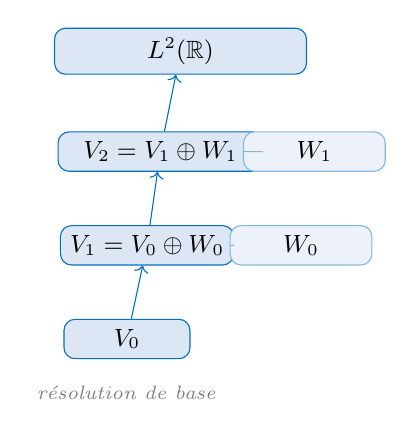
\begin{tikzpicture}[scale=0.85, font=\small]
				\node[draw=bleu, fill=bleulight, rounded corners,
				minimum width=3.2cm, minimum height=0.5cm]
				(L2) at (1.6,5.5) {$L^2(\RR)$};
				
				\node[draw=bleu, fill=bleulight, rounded corners,
				minimum width=2.6cm, minimum height=0.5cm]
				(V2) at (1.3,4.0) {$V_2 = V_1 \oplus W_1$};
				\node[draw=bleu!50, fill=bleulight!50, rounded corners,
				minimum width=1.8cm, minimum height=0.5cm]
				(W1) at (3.6,4.0) {$W_1$};
				
				\node[draw=bleu, fill=bleulight, rounded corners,
				minimum width=2.2cm, minimum height=0.5cm]
				(V1) at (1.1,2.6) {$V_1 = V_0 \oplus W_0$};
				\node[draw=bleu!50, fill=bleulight!50, rounded corners,
				minimum width=1.8cm, minimum height=0.5cm]
				(W0b) at (3.4,2.6) {$W_0$};
				
				\node[draw=bleu, fill=bleulight, rounded corners,
				minimum width=1.6cm, minimum height=0.5cm]
				(V0) at (0.8,1.2) {$V_0$};
				\node[font=\scriptsize, gris] at (0.8,0.4) {\textit{résolution de base}};
				
				\draw[->, bleu] (V0) -- (V1);
				\draw[->, bleu] (V1) -- (V2);
				\draw[->, bleu] (V2) -- (L2);
				\draw[bleu!50] (W0b) -- (V1);
				\draw[bleu!50] (W1) -- (V2);
			\end{tikzpicture}
			
		\end{columns}
		
	\end{frame}
	
	% ─────────────────────────────────────────────────────────────────────────
	\begin{frame}{III — L'équation de raffinement}
		
		La fonction d'échelle $\varphi \in V_0 \subset V_1$, donc elle se décompose
		dans la base $\{\sqrt{2}\,\varphi(2\cdot - n)\}$ de $V_1$ :
		\[
		\boxed{\varphi(x) = \sqrt{2} \sum_{n \in \ZZ} h_n\, \varphi(2x - n)}
		\]
		Les coefficients $(h_n)$ définissent le \textbf{filtre passe-bas discret}.
		
		\medskip
		L'ondelette est construite à partir de $\varphi$ par les
		\textbf{coefficients miroir en quadrature} :
		\[
		\boxed{\psi(x) = \sqrt{2} \sum_{n \in \ZZ} g_n\, \varphi(2x - n),}
		\qquad
		g_n = (-1)^{1-n}\, h_{1-n}
		\]
		Les $(g_n)$ définissent le \textbf{filtre passe-haut discret}.
		
		\medskip
		\begin{block}{Exemple — Haar}
			$h_0 = h_1 = \tfrac{1}{\sqrt{2}}$ \quad (moyenne) \qquad
			$g_0 = \tfrac{1}{\sqrt{2}},\; g_1 = -\tfrac{1}{\sqrt{2}}$ \quad (différence)
		\end{block}
		
		\medskip
		\textbf{Condition d'orthogonalité} : $\sum_n h_n h_{n-2k} = \delta_{0,k}$
		(les filtres $h$ et $g$ sont orthogonaux et normalisés).
		
	\end{frame}
	
	% ════════════════════════════════════════════════════════════════════════
	\section{IV. Algorithmes et transformée discrète (DWT)}
	% ════════════════════════════════════════════════════════════════════════
	
	\begin{frame}{IV — Le banc de filtres de Mallat}
		
		\begin{block}{Algorithme pyramidal de Mallat (1989)}
			Les coefficients au niveau $j$ se calculent à partir du niveau $j+1$
			par un \textbf{filtrage suivi d'un sous-échantillonnage} $\downarrow 2$ :
			\[
			c_{j,k} = \sum_n h_{n-2k}\, c_{j+1,n}, \qquad
			d_{j,k} = \sum_n g_{n-2k}\, c_{j+1,n}
			\]
		\end{block}
		
		\begin{center}
			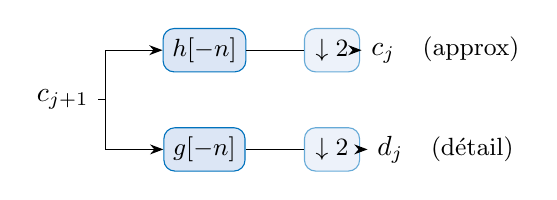
\begin{tikzpicture}[
				scale=0.9,
				box/.style={draw=bleu, fill=bleulight, rounded corners,
					minimum width=1.0cm, minimum height=0.55cm,
					font=\small, text centered},
				ds/.style={draw=bleu!60, fill=bleulight!50, rounded corners,
					minimum width=0.7cm, minimum height=0.55cm,
					font=\small, text centered},
				>=Stealth
				]
				\node (x) at (0,0) {$c_{j+1}$};
				\node[box] (h) at (2.0,0.7)  {$h[-n]$};
				\node[box] (g) at (2.0,-0.7) {$g[-n]$};
				\node[ds]  (d2h) at (3.8,0.7)  {$\downarrow 2$};
				\node[ds]  (d2g) at (3.8,-0.7) {$\downarrow 2$};
				\node (cj)  at (5.4,0.7)  {$c_j$\quad\small(approx)};
				\node (dj)  at (5.4,-0.7) {$d_j$\quad\small(détail)};
				
				\draw[->] (x) -- ++(0.6,0) |- (h);
				\draw[->] (x) -- ++(0.6,0) |- (g);
				\draw[->] (h) -- (d2h) -- (cj);
				\draw[->] (g) -- (d2g) -- (dj);
			\end{tikzpicture}
		\end{center}
		
		\medskip
		\textbf{Filtrage = produit scalaire} : chaque $c_{j,k}$ est la projection
		orthogonale de $c_{j+1}$ sur $\varphi_{j,k}$, et chaque $d_{j,k}$
		sur $\psi_{j,k}$.
		
		\medskip
		\textbf{Complexité} : $\mathcal{O}(N)$ par niveau, $\mathcal{O}(N \log N)$
		en tout — comparable à la FFT.
		
	\end{frame}
	
	% ─────────────────────────────────────────────────────────────────────────
	\begin{frame}{IV — Le cas de Haar : moyennes et différences}
		
		Pour Haar, les filtres ont seulement deux coefficients :
		
		\[
		h = \tfrac{1}{\sqrt{2}}\begin{pmatrix}1\\1\end{pmatrix}, \quad
		g = \tfrac{1}{\sqrt{2}}\begin{pmatrix}1\\-1\end{pmatrix}
		\]
		
		\medskip
		\textbf{Opération sur une paire $(a, b)$ :}
		\[
		\underbrace{\frac{a+b}{\sqrt{2}}}_{\text{approximation}} \qquad
		\underbrace{\frac{a-b}{\sqrt{2}}}_{\text{détail}}
		\]
		
		\medskip
		\textbf{Exemple complet sur 8 valeurs (3 niveaux) :}
		\[
		\underbrace{[2\;4\;8\;12\;14\;0\;2\;1]}_{N=8}
		\;\xrightarrow{\text{niv.1}}\;
		\underbrace{[3\;10\;7\;1.5]}_{\text{approx}} \,|\, [-1\;{-2}\;7\;0.5]
		\;\xrightarrow{\text{niv.2}}\;
		[6.5\;4.25]\,|\,[-3.5\;2.75]\,|\,\cdots
		\;\xrightarrow{\text{niv.3}}\;
		[5.4\,|\,1.1\,|\,\cdots]
		\]
		
		\medskip
		\begin{block}{Conservation de l'énergie}
			$\left(\dfrac{a+b}{\sqrt{2}}\right)^2 + \left(\dfrac{a-b}{\sqrt{2}}\right)^2
			= a^2 + b^2$
			\quad $\Rightarrow$ $\norme{Mx}^2 = \norme{x}^2$
			\quad ($M$ est orthogonale).
		\end{block}
		
	\end{frame}
	
	% ─────────────────────────────────────────────────────────────────────────
	\begin{frame}{IV — La matrice de Haar : une matrice orthogonale}
		
		La transformée sur un signal de longueur $N=8$ s'écrit $y = Mx$ où :
		
		\[
		M = \frac{1}{\sqrt{2}}
		\begin{pmatrix}
			1 & 1 & 0 & 0 & 0 & 0 & 0 & 0 \\
			0 & 0 & 1 & 1 & 0 & 0 & 0 & 0 \\
			0 & 0 & 0 & 0 & 1 & 1 & 0 & 0 \\
			0 & 0 & 0 & 0 & 0 & 0 & 1 & 1 \\
			1 &-1 & 0 & 0 & 0 & 0 & 0 & 0 \\
			0 & 0 & 1 &-1 & 0 & 0 & 0 & 0 \\
			0 & 0 & 0 & 0 & 1 &-1 & 0 & 0 \\
			0 & 0 & 0 & 0 & 0 & 0 & 1 &-1 \\
		\end{pmatrix}
		\]
		
		\medskip
		Chaque \textbf{ligne est un vecteur de base} : les lignes du haut projettent
		sur les translations de $\varphi_{1,k}$ (approximation), les lignes du bas
		sur $\psi_{1,k}$ (détail).
		
		\medskip
		\begin{alertblock}{Résultat clé (MP — algèbre linéaire)}
			$M^\top M = I$ (orthogonale) $\Rightarrow$ l'inverse est la transposée :
			$M^{-1} = M^\top$.
			La reconstruction est immédiate et la décomposition est \emph{sans perte}.
		\end{alertblock}
		
	\end{frame}
	
	% ─────────────────────────────────────────────────────────────────────────
	\begin{frame}{IV — Généralisation 2D : l'algorithme de Mallat}
		
		Une image $F[n,m]$ est une fonction de $\RR^2$. On exploite la
		\textbf{séparabilité} : base $2\mathrm{D}$ = produit tensoriel de deux bases $1\mathrm{D}$.
		
		\medskip
		\textbf{Application successive sur les lignes puis les colonnes :}
		
		\begin{center}
			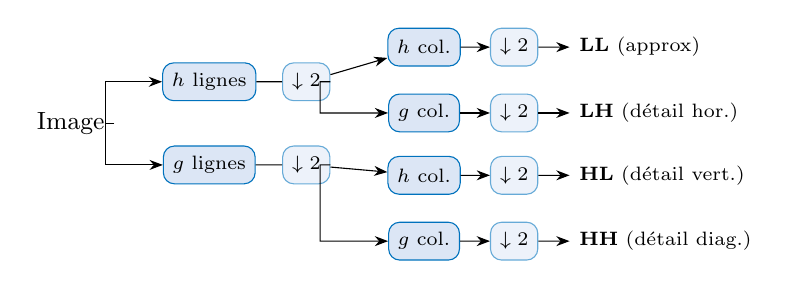
\begin{tikzpicture}[scale=0.88,
				>=Stealth,
				box/.style={draw=bleu, fill=bleulight, rounded corners,
					minimum width=0.85cm, minimum height=0.48cm,
					font=\scriptsize, text centered},
				ds/.style={draw=bleu!60, fill=bleulight!50, rounded corners,
					minimum width=0.6cm, minimum height=0.48cm,
					font=\scriptsize}
				]
				\node[font=\small] (im) at (0,0) {Image};
				
				% Sur les lignes
				\node[box] (hl) at (2.0,0.6) {$h$ lignes};
				\node[box] (gl) at (2.0,-0.6) {$g$ lignes};
				\node[ds]  (dl2h) at (3.4,0.6) {$\downarrow 2$};
				\node[ds]  (dl2g) at (3.4,-0.6) {$\downarrow 2$};
				
				% Sur les colonnes (chacune)
				\node[box] (hhc) at (5.1,1.1) {$h$ col.};
				\node[box] (hgc) at (5.1,0.15) {$g$ col.};
				\node[box] (ghc) at (5.1,-0.75) {$h$ col.};
				\node[box] (ggc) at (5.1,-1.7) {$g$ col.};
				
				\node[ds] (ds1) at (6.4,1.1) {$\downarrow 2$};
				\node[ds] (ds2) at (6.4,0.15) {$\downarrow 2$};
				\node[ds] (ds3) at (6.4,-0.75) {$\downarrow 2$};
				\node[ds] (ds4) at (6.4,-1.7) {$\downarrow 2$};
				
				\node[font=\scriptsize, right] (LL) at (7.2,1.1)  {\textbf{LL} (approx)};
				\node[font=\scriptsize, right] (LH) at (7.2,0.15) {\textbf{LH} (détail hor.)};
				\node[font=\scriptsize, right] (HL) at (7.2,-0.75) {\textbf{HL} (détail vert.)};
				\node[font=\scriptsize, right] (HH) at (7.2,-1.7)  {\textbf{HH} (détail diag.)};
				
				\draw[->] (im) -- ++(0.5,0) |- (hl);
				\draw[->] (im) -- ++(0.5,0) |- (gl);
				\draw[->] (hl) -- (dl2h) -- (hhc);
				\draw[->] (dl2h) -- ++(0.2,0) |- (hgc);
				\draw[->] (gl) -- (dl2g) -- (ghc);
				\draw[->] (dl2g) -- ++(0.2,0) |- (ggc);
				\foreach \a/\b in {hhc/ds1, hgc/ds2, ghc/ds3, ggc/ds4}
				\draw[->] (\a) -- (\b);
				\foreach \a/\b in {ds1/LL, ds2/LH, ds3/HL, ds4/HH}
				\draw[->] (\a) -- (\b);
			\end{tikzpicture}
		\end{center}
		
		\medskip
		On itère sur la sous-bande \textbf{LL} pour les niveaux suivants.
		
	\end{frame}
	
	% ─────────────────────────────────────────────────────────────────────────
	\begin{frame}{IV — Représentation en mémoire après $L$ niveaux}
		
		Pour une image $N \times N$ et $L = 3$ niveaux de décomposition :
		
		\medskip
		\begin{center}
			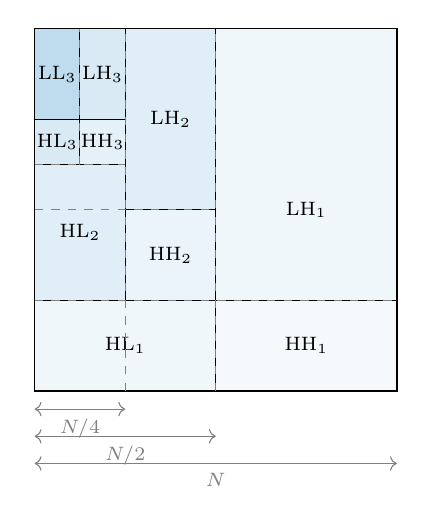
\begin{tikzpicture}[scale=1.15, font=\scriptsize]
				
				\draw[fill=white, draw=black, thick] (0,0) rectangle (4,4);
				
				% Niveau 3 (quart haut-gauche du bloc 16×16)
				\draw[fill=bleu!25]     (0,3) rectangle (0.5,4)   node[midway] {LL$_3$};
				\draw[fill=bleu!15]     (0.5,3) rectangle (1,4)   node[midway] {LH$_3$};
				\draw[fill=bleu!15]     (0,2.5) rectangle (0.5,3) node[midway] {HL$_3$};
				\draw[fill=bleu!10]     (0.5,2.5) rectangle (1,3) node[midway] {HH$_3$};
				
				% Niveau 2 (bloc 16×16, hors coin déjà dessiné)
				\draw[fill=bleu!12]     (1,2) rectangle (2,4)     node[midway] {LH$_2$};
				\draw[fill=bleu!12]     (0,1) rectangle (1,2.5)   node[midway] {HL$_2$};
				\draw[fill=bleu!08]     (1,1) rectangle (2,2)     node[midway] {HH$_2$};
				
				% Niveau 1
				\draw[fill=bleu!06]     (2,0) rectangle (4,4)     node[midway] {LH$_1$};
				\draw[fill=bleu!06]     (0,0) rectangle (2,1)     node[midway] {HL$_1$};
				\draw[fill=bleu!04]     (2,0) rectangle (4,1)     node[midway] {HH$_1$};
				
				% Quadrillage
				\draw[dashed, gris, thin] (1,0)--(1,4);
				\draw[dashed, gris, thin] (2,0)--(2,4);
				\draw[dashed, gris, thin] (0,1)--(4,1);
				\draw[dashed, gris, thin] (0,2)--(2,2);
				\draw[dashed, gris, thin] (0,2.5)--(1,2.5);
				\draw[dashed, gris, thin] (0.5,2.5)--(0.5,4);
				
				% Annotations
				\draw[<->, gris, thin] (0,-0.2) -- (1,-0.2) node[midway, below] {$N/4$};
				\draw[<->, gris, thin] (0,-0.5) -- (2,-0.5) node[midway, below] {$N/2$};
				\draw[<->, gris, thin] (0,-0.8) -- (4,-0.8) node[midway, below] {$N$};
				
			\end{tikzpicture}
		\end{center}
		
	\end{frame}
	
	% ─────────────────────────────────────────────────────────────────────────
	\begin{frame}[fragile]{IV — Implémentation Python}
		
		\begin{columns}[T]
			\column{0.50\textwidth}
			
			\begin{lstlisting}
				class Haar(BaseOndelette):
				def __init__(self, img, levels):
				super().__init__(img, levels)
				s2 = np.sqrt(2)
				self.h = np.array([1/s2, 1/s2])
				self.g = np.array([1/s2,-1/s2])
				
				def t1d(self, x):
				n, L = len(x), len(self.h)
				xp = np.pad_circular(x, L)
				out = np.zeros(n)
				for i in range(n//2):
				seg = xp[2*i:2*i+L]
				out[i]       = seg @ self.h
				out[i+n//2]  = seg @ self.g
				return out
			\end{lstlisting}
			
			\column{0.46\textwidth}
			
			\begin{lstlisting}
				def forward(self):
				res = self.img.copy()
				n, p = res.shape
				for _ in range(self.levels):
				res[:n,:p] = self.t2d(
				res[:n,:p])
				n //= 2; p //= 2
				return res
				
				def inverse(self, coeffs):
				res = coeffs.copy()
				n = len(res)
				n //= 2**(self.levels-1)
				for _ in range(self.levels):
				res[:n,:n] = self.t2d_inv(
				res[:n,:n])
				n *= 2
				return res
			\end{lstlisting}
			
		\end{columns}
		
	\end{frame}
	
	% ════════════════════════════════════════════════════════════════════════
	\section{V. Application : compression d'image}
	% ════════════════════════════════════════════════════════════════════════
	
	\begin{frame}{V — Principe du codeur par transformée}
		
		\begin{block}{Étapes de la compression}
			\begin{enumerate}
				\item \textbf{Transformée} : $F \mapsto \{c_{j,k},\, d_{j,k}\}$
				(base hilbertienne de $L^2$)
				\item \textbf{Seuillage} des coefficients de détail :
				\[
				\bar{d}_{j,k} =
				\begin{cases}
					d_{j,k} & \text{si } |d_{j,k}| \geq \lambda \\
					0        & \text{sinon}
				\end{cases}
				\qquad \text{(seuillage \emph{dur})}
				\]
				\item \textbf{Reconstruction} : $\bar{F} = \sum_{j,k} \bar{d}_{j,k}\,\psi_{j,k}$
				\item \textbf{Erreur} (identité de Parseval) :
				\[
				\norme{F - \bar{F}}^2 = \sum_{\substack{j,k\\|\bar{d}_{j,k}|=0}} d_{j,k}^2
				\]
			\end{enumerate}
		\end{block}
		
		\medskip
		Seuls les coefficients mis à zéro contribuent à l'erreur — et les
		coefficients petits correspondant aux zones \emph{lisses} de l'image
		peuvent être éliminés sans dégradation perceptible.
		
	\end{frame}
	
	% ─────────────────────────────────────────────────────────────────────────
	\begin{frame}{V — Seuillage dur et seuil optimal}
		
		\begin{columns}[T]
			\column{0.50\textwidth}
			
			\textbf{Deux modes de seuillage :}
			
			\medskip
			\emph{Dur} : discontinu en $\lambda$,
			conserve l'amplitude des grands coefficients.
			\[
			\bar{c} =
			\begin{cases} c & |c| \geq \lambda \\ 0 & |c| < \lambda \end{cases}
			\]
			
			\emph{Doux} : continu, réduit tous les coefficients vers zéro.
			\[
			\bar{c} = \mathrm{sgn}(c)\max(|c| - \lambda, 0)
			\]
			
			\medskip
			\begin{block}{Seuil de Donoho (1994)}
				Pour un bruit additif gaussien $\mathcal{N}(0,\sigma^2)$ :
				\[
				\lambda^* = \sigma\sqrt{2 \ln N}
				\]
				Estimateur minimax optimal.
			\end{block}
			
			\column{0.46\textwidth}
			
			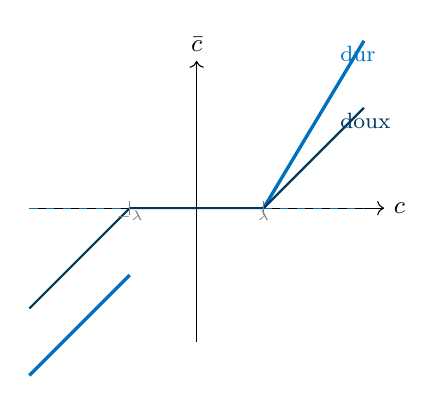
\begin{tikzpicture}[scale=0.85]
				\draw[->] (-2.5,0) -- (2.8,0) node[right] {\small $c$};
				\draw[->] (0,-2.0) -- (0,2.2) node[above] {\small $\bar{c}$};
				% seuillage dur
				\draw[bleu, very thick]
				(-2.5,-2.5) -- (-1,-1) (-1,0) (-1,-1)
				(1,0) -- (2.5,2.5);
				\draw[bleu, dashed]
				(-2.5,0) -- (-1,0);
				\draw[bleu, dashed]
				(1,0) -- (2.5,0);
				% seuillage doux
				\draw[bleu!50!black, thick]
				(-2.5,-1.5) -- (-1,0) -- (1,0) -- (2.5,1.5);
				% légendes
				\node[bleu, font=\footnotesize, right] at (2.0,2.3) {dur};
				\node[bleu!50!black, font=\footnotesize, right] at (2.0,1.3) {doux};
				% traits lambda
				\draw[gris, thin] (1,-0.1) -- (1,0.1) node[below, font=\tiny] {$\lambda$};
				\draw[gris, thin] (-1,-0.1) -- (-1,0.1) node[below, font=\tiny] {$-\lambda$};
			\end{tikzpicture}
			
		\end{columns}
		
	\end{frame}
	
	% ─────────────────────────────────────────────────────────────────────────
	\begin{frame}{V — Résultats expérimentaux}
		
		\begin{columns}[T]
			\column{0.50\textwidth}
			
			\textbf{Configuration} :
			\begin{itemize}
				\item Image RGB $512 \times 512$
				\item Ondelette de Haar, $L = 3$ niveaux
				\item Seuillage dur, seuil $\lambda$ variable
			\end{itemize}
			
			\medskip
			\begin{center}
				\begin{tabular}{@{}rcc@{}}
					\toprule
					$\lambda$ & Compression $\tau$ & PSNR \\
					\midrule
					0          & $0\,\%$   & $+\infty$ \\
					10         & $23\,\%$  & 43 dB \\
					20         & $45\,\%$  & 38 dB \\
					40         & $70\,\%$  & 32 dB \\
					80         & $88\,\%$  & 27 dB \\
					\bottomrule
				\end{tabular}
			\end{center}
			
			\medskip
			{\small $\tau = \#\{c : |c| < \lambda\} / N^2$,\;
				$\mathrm{PSNR} = 10\log_{10}\!\tfrac{255^2}{\mathrm{MSE}}$}
			
			\column{0.46\textwidth}
			
			\textbf{Courbe PSNR vs compression}
			
			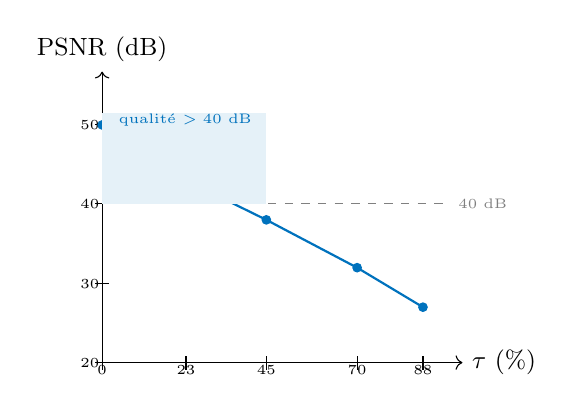
\begin{tikzpicture}[scale=0.88]
				\draw[->] (0,0) -- (5.2,0) node[right] {\small $\tau$ (\%)};
				\draw[->] (0,0) -- (0,4.2) node[above] {\small PSNR (dB)};
				% axes labels
				\foreach \xv/\xl in {0/0, 1.21/23, 2.37/45, 3.68/70, 4.63/88}
				\draw (\xv,-0.1) -- (\xv,0.1) node[below,font=\tiny] {\xl};
				\foreach \yv/\yl in {0/20, 1.14/30, 2.29/40, 3.43/50}
				\draw (-0.1,\yv) -- (0.1,\yv) node[left,font=\tiny] {\yl};
				% seuil 40 dB
				\draw[gris, dashed, thin] (0,2.29) -- (5.0,2.29)
				node[right, font=\tiny, gris] {40 dB};
				% courbe
				\draw[bleu, thick]
				(0.00,3.43)--(1.21,2.63)--(2.37,2.06)--(3.68,1.37)--(4.63,0.80);
				\foreach \px/\py in {0.00/3.43, 1.21/2.63, 2.37/2.06, 3.68/1.37, 4.63/0.80}
				\fill[bleu] (\px,\py) circle (2pt);
				% zone bonne qualité
				\fill[bleu!10] (0,2.29) rectangle (2.37,3.6);
				\node[bleu, font=\tiny] at (1.2,3.5) {qualité $> 40$ dB};
			\end{tikzpicture}
			
			\medskip
			{\small Jusqu'à $\approx 45\,\%$ de compression
				avec une qualité excellente.}
			
		\end{columns}
		
	\end{frame}
	
	% ─────────────────────────────────────────────────────────────────────────
	\begin{frame}{V — Intérêt des moments nuls}
		
		\begin{block}{Propriété de décroissance des coefficients}
			Si $\psi$ a $N$ moments nuls ($\int x^n \psi(x)\d x = 0$ pour $n < N$)
			et si $f \in \mathcal{C}^N$ au voisinage de $x_0$, alors :
			\[
			|d_{j,k}| \leq C\, 2^{-j(N + 1/2)}
			\quad \text{pour } k \cdot 2^{-j} \text{ proche de } x_0
			\]
		\end{block}
		
		\begin{columns}[T]
			\column{0.50\textwidth}
			
			\medskip
			\textbf{Conséquence pour la compression} :
			plus $N$ est grand, plus les coefficients sur les zones
			lisses de l'image \emph{décroissent vite} avec l'échelle
			$\Rightarrow$ seuillage plus agressif possible.
			
			\medskip
			\begin{center}
				\begin{tabular}{@{}lcc@{}}
					\toprule
					& Haar & Daubechies D4 \\
					\midrule
					Moments nuls    & 1 & 2 \\
					Support         & 2 & 4 \\
					PSNR @ 45\%     & 38 dB & 41 dB \\
					\bottomrule
				\end{tabular}
			\end{center}
			
			\column{0.46\textwidth}
			
			\textbf{JPEG\,2000} utilise les ondelettes CDF~9/7
			(biorthogonales, 4 moments nuls) :
			
			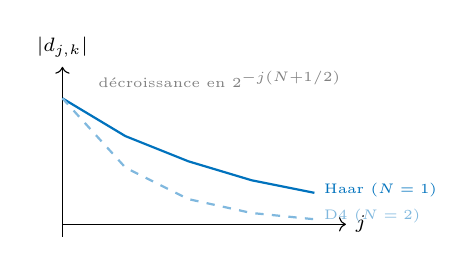
\begin{tikzpicture}[scale=0.8, font=\scriptsize]
				% Haar : 1 moment nul -> coefficients décroissent lentement
				\draw[->] (0,0) -- (4.5,0) node[right] {$j$};
				\draw[->] (0,-0.2) -- (0,2.5) node[above] {$|d_{j,k}|$};
				\draw[bleu, thick]
				(0,2.0) -- (1,1.4) -- (2,1.0) -- (3,0.7) -- (4,0.5);
				\draw[bleu!50, thick, dashed]
				(0,2.0) -- (1,0.9) -- (2,0.4) -- (3,0.18) -- (4,0.08);
				\node[bleu, font=\tiny, right] at (4,0.55) {Haar ($N=1$)};
				\node[bleu!50, font=\tiny, right] at (4,0.13) {D4 ($N=2$)};
				\node[font=\tiny, gris] at (2.5,2.3) {décroissance en $2^{-j(N+1/2)}$};
			\end{tikzpicture}
			
		\end{columns}
		
	\end{frame}
	
	% ════════════════════════════════════════════════════════════════════════
	\section{VI. Conclusion}
	% ════════════════════════════════════════════════════════════════════════
	
	\begin{frame}{VI — Bilan : les atouts des ondelettes}
		
		\begin{columns}[T]
			\column{0.50\textwidth}
			
			\begin{block}{Localisation temps-fréquence}
				Contrairement à Fourier, chaque coefficient $d_{j,k}$
				est lié à une \emph{position} et une \emph{échelle} précises.
				Les singularités de l'image sont identifiées localement.
			\end{block}
			
			\medskip
			
			\begin{block}{Orthogonalité et conservation de l'énergie}
				La matrice $M$ est orthogonale ($M^\top M = I$) :
				\begin{itemize}
					\item Reconstruction exacte : $M^{-1} = M^\top$
					\item Parseval discret : $\norme{Mx}^2 = \norme{x}^2$
					\item L'erreur de compression est directement calculable
				\end{itemize}
			\end{block}
			
			\column{0.46\textwidth}
			
			\begin{block}{Efficacité algorithmique}
				Algorithme de Mallat :
				\begin{itemize}
					\item $\mathcal{O}(N^2)$ pour une image $N \times N$
					\item Inférieur à la FFT 2D en $\mathcal{O}(N^2 \log N)$
					\item Implémentation naturelle par filtrage séparable
				\end{itemize}
			\end{block}
			
			\medskip
			
			\begin{block}{Lien avec le programme}
				Espaces de Hilbert, bases orthonormées, matrices orthogonales,
				convolution discrète, estimateurs statistiques (Donoho).
			\end{block}
			
		\end{columns}
		
	\end{frame}
	
	% ─────────────────────────────────────────────────────────────────────────
	\begin{frame}{VI — Ouverture}
		
		\begin{columns}[T]
			\column{0.50\textwidth}
			
			\textbf{JPEG\,2000 et le standard actuel}
			
			\medskip
			Le format JPEG\,2000 remplace la DCT par blocs de JPEG
			par une DWT globale avec les ondelettes \emph{CDF 9/7}
			(Cohen--Daubechies--Feauveau, biorthogonales).
			
			Avantages : pas d'artefacts de blocs, compression progressive,
			scalabilité de la résolution.
			
			\medskip
			\textbf{Au-delà de la compression}
			
			\medskip
			Les ondelettes sont utilisées en :
			\begin{itemize}
				\item Débruitage (seuillage doux adaptatif)
				\item Analyse de turbulence (détection de tourbillons)
				\item Traitement du signal médical (EEG, IRM)
				\item Tatouage numérique (watermarking)
			\end{itemize}
			
			\column{0.46\textwidth}
			
			\textbf{Comparaison JPEG / JPEG\,2000}
			
			\medskip
			\begin{center}
				\begin{tabular}{@{}lcc@{}}
					\toprule
					& JPEG       & JPEG\,2000 \\
					\midrule
					Base       & DCT        & DWT        \\
					Blocs      & $8\times8$ & global     \\
					Artefacts  & blocs      & flou doux  \\
					Moments    & ---        & 4          \\
					\bottomrule
				\end{tabular}
			\end{center}
			
			\medskip
			\begin{alertblock}{Pour aller plus loin}
				Ondelettes biorthogonales (CDF), paquets d'ondelettes,
				transformées en curvelets pour les images naturelles.
			\end{alertblock}
			
		\end{columns}
		
	\end{frame}
	
	% ─────────────────────────────────────────────────────────────────────────
	\begin{frame}{}
		\begin{center}
			\vspace{1.5cm}
			{\Large\bfseries Merci pour votre attention.}
			
			\vspace{1.5cm}
			{\large Questions ?}
			
			\vspace{1.5cm}
			{\small
				\textit{Sources :}\\
				V.\ Perrier, \textit{Applications de la théorie des ondelettes}, IMAG 2005.\\
				S.\ Mallat, \textit{Une exploration des signaux en ondelettes}, \'Ed.\ Polytechnique, 2000.}
		\end{center}
	\end{frame}
	
	% ────────────────────────────────────────────────────────────────────────
	% ANNEXES
	% ────────────────────────────────────────────────────────────────────────
	
	\appendix
	
	\begin{frame}[fragile]{Annexe — Implémentation complète de l'inverse}
		
		\begin{lstlisting}
			def inverse(self, coeffs):
			"""
			Reconstruction multi-niveaux.
			Démarre à N//2^(L-1) : le bloc de niveau L contient
			LL_L et ses 3 sous-bandes de détail dans les quadrants
			adjacents. On ne peut pas reconstruire avec LL_L seul.
			"""
			res = coeffs.copy()
			n, p = res.shape
			n //= 2 ** (self.levels - 1)   # taille de départ correcte
			p //= 2 ** (self.levels - 1)
			for _ in range(self.levels):
			res[:n, :p] = self.transformation_2d_inverse(res[:n, :p])
			n *= 2
			p *= 2
			return res
		\end{lstlisting}
		
	\end{frame}
	
	% ─────────────────────────────────────────────────────────────────────────
	\begin{frame}{Annexe — Pourquoi $N / 2^{L-1}$ et non $N / 2^L$ ?}
		
		\begin{columns}[T]
			\column{0.55\textwidth}
			
			Après $L$ niveaux, le contenu mémoire est :
			\begin{itemize}
				\item Le coin $\tfrac{N}{2^L} \times \tfrac{N}{2^L}$ contient \textbf{LL}$_L$ seul.
				\item Pour inverser le niveau $L$, il faut les \textbf{quatre quadrants}
				du bloc $\tfrac{N}{2^{L-1}} \times \tfrac{N}{2^{L-1}}$ :
				LL$_L$, LH$_L$, HL$_L$, HH$_L$.
			\end{itemize}
			
			\medskip
			\textbf{Erreur classique} : démarrer à $N/2^L$ (ne voir que LL$_L$)
			$\Rightarrow$ reconstruction corrompue, les détails du niveau $L$
			sont ignorés.
			
			\medskip
			\textbf{Règle} : la taille de la fenêtre de travail à l'itération $\ell$
			de l'inverse est :
			\[
			n_\ell = \frac{N}{2^{L-\ell}}, \quad \ell = 1, \ldots, L
			\]
			
			\column{0.42\textwidth}
			
			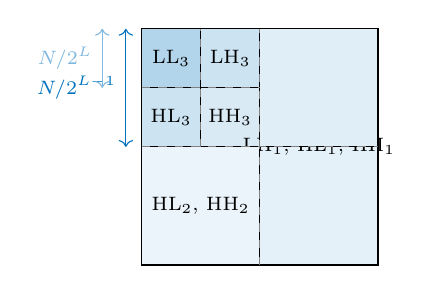
\begin{tikzpicture}[scale=1.0, font=\scriptsize]
				\draw[fill=white, draw=black, thick] (0,0) rectangle (3,3);
				
				\draw[fill=bleu!30] (0,2.25) rectangle (0.75,3) node[midway] {LL$_3$};
				\draw[fill=bleu!20] (0.75,2.25) rectangle (1.5,3) node[midway] {LH$_3$};
				\draw[fill=bleu!20] (0,1.5) rectangle (0.75,2.25) node[midway] {HL$_3$};
				\draw[fill=bleu!15] (0.75,1.5) rectangle (1.5,2.25) node[midway] {HH$_3$};
				
				\draw[fill=bleu!10] (1.5,0) rectangle (3,3) node[midway] {LH$_1$, HL$_1$, HH$_1$};
				\draw[fill=bleu!08] (0,0) rectangle (1.5,1.5) node[midway] {HL$_2$, HH$_2$};
				\draw[fill=bleu!12] (1.5,1.5) rectangle (3,3) node[midway] {};
				
				\draw[dashed, gris] (1.5,0)--(1.5,3);
				\draw[dashed, gris] (0,1.5)--(3,1.5);
				\draw[dashed, gris] (0,2.25)--(1.5,2.25);
				\draw[dashed, gris] (0.75,1.5)--(0.75,3);
				
				% Accolade N/2^(L-1)
				\draw[<->, bleu, thin] (-0.2,1.5) -- (-0.2,3)
				node[midway, left] {$N/2^{L-1}$};
				\draw[<->, bleu!50, thin] (-0.5,2.25) -- (-0.5,3)
				node[midway, left] {$N/2^L$};
			\end{tikzpicture}
			
		\end{columns}
		
	\end{frame}
	
\end{document}